\documentclass[a4paper,10pt]{article}
\usepackage[utf8]{inputenc}
\usepackage{lmodern}
\usepackage[T1]{fontenc}
\usepackage[italian]{babel}
\usepackage{graphicx}
\usepackage{listings}
\usepackage{color}
\usepackage{geometry}
\geometry{a4paper, left=1.5cm, right=1.5cm, top=2.5cm, bottom=2cm}
\definecolor{lightgray}{gray}{0.9}
\setlength{\parindent}{5mm}
\linespread{1}

 

\begin{document}
	
	\title{Programmazione ad Oggetti\\Relazione progetto Kalk}
	\author{Daniel Rossi\\Matricola 1125444}
	\date{}
	\maketitle
	\begin{figure}[!h]
		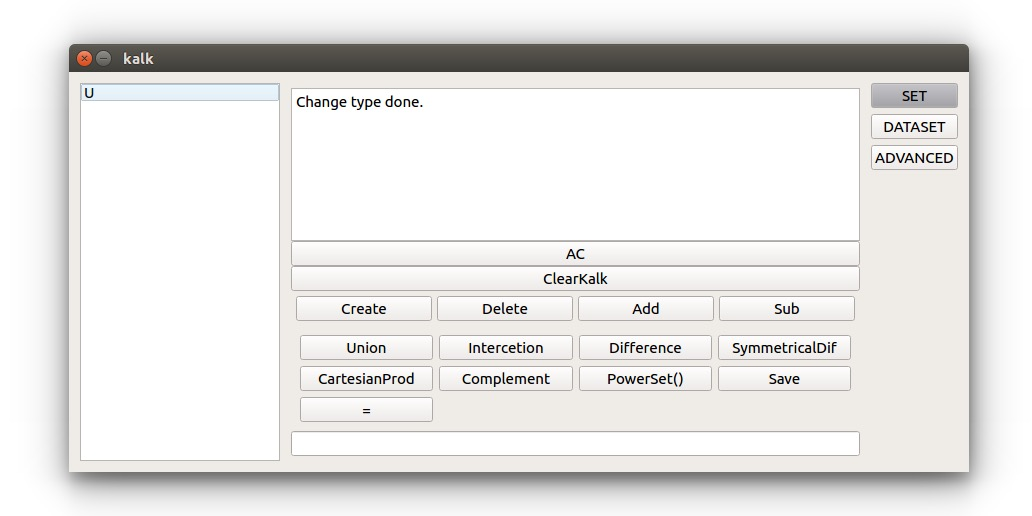
\includegraphics[scale=0.5]{img/kalk.jpg}
			\caption{Schermata di default Kalk}
    \end{figure}
    \newpage
	\tableofcontents
	\newpage
	
	\section{Scopo del Progetto}
	Il progetto si prefiggeva la realizzazione di una calcolatrice che operasse su diversi tipi di dato numerico. I dati disponibili nella calcolatrice sono: gli insiemi numerici interi detti “SET”, questi permettono di eseguire le principali operazioni insiemistiche tra insiemi inseriti in un insieme universo detto \textit{U}, con la possibilità di salvarne il risultato, ogni SET conterrà come impone la teoria degli insiemi una sola istanza dello stesso valore; i DATASET comuni sono insiemi campionari di numeri interi che posso comparire anche più volte nello stesso DATASET, questi rappresentano una sequenza di misurazioni intere e forniscono le principali operazioni statistiche su un determinato insieme campionario, come media varianza e deviazione standard; gli ADVANCED dataset sono dataset con valori compresi nell’intervallo [-50 , +50], questi insiemi campionari sono pensati per essere messi in relazione tra loro per ricavare informazioni sulla correlazione dei due insiemi stessi. La calcolatrice è divisa in tre schede, una per ogni tipo di dato, ci si prefiggeva di avere schede diverse per ogni insieme.

	\section{Gerarchie utilizzate}
	\subsection{Gerarchia dei tipi di dato}
	\subsubsection{Class Numbers}
	La classe astratta Numbers rappresenta un’ipotetica sequenza di numeri interi. Numbers ha un campo dati di tipo stringa che identifica ciascuna sequenza di numeri, definisce inoltre diversi metodi virtuali puri di clonazione e di aggiunta e rimozione di interi dalle liste.
    Inoltre definisce i seguenti metodi per la lettura e scrittura del nome del \textit{Numbers}.
    La classe \textit{Numbers} una classe annidata protetta \textit{Ris}, utilizzata per operazioni di ricerca sempre dalle classi derivate.
    
    \subsubsection{Class Set}
    La classe concreta \textit{Set}, derivata dalla classe astratta \textit{Numbers}, rappresenta un insieme numerico di interi univoci dove l’ordine con cui vengono inseriti non ha alcuna importanza. 
    Implementa i metodi virtuali della classe \textit{Numbers}:
	\begin{itemize}
        \item \textbf{set* clone() const}: resistuisce una copia dell'oggetto di invocazione \textit{Set};
		\item \textbf{std::string name() const}: restituisce la stringa \textit{set};
        \item \textbf{void add\_value(const int)}: aggiunge un intero all'oggetto \textit{Set} se non è già presente;
		\item \textbf{void sub\_value(const int)}: sottrae un intero all'oggetto \textit{Set};
		\item \textbf{void add\_list(const std::list<int>\&)}: aggiunge un lista di interi all'oggetto \textit{Set} se non sono già presenti;
        \item \textbf{void sub\_list(const std::list<int>\&)}: sottrae una lista di interi all'oggetto \textit{Set};
    \end{itemize}
    Dispone di metodi propri per la lettura e scrittura della lista di interi, inoltre viene fatto l'overloading  degli operatori:
    Esegue l'overloading dei seguenti metodi propri tra cui  quelli più importanti:
    \begin{itemize}
        \item operator std::string()
        \item set\& operator+(const set\&) const
        \item set\& operator-(const set\&) const
        \item set\& operator/(const set\&) const
    \end{itemize}

    \subsubsection{Class Dataset}
    La classe concreta \textit{Dataset}, derivata dalla classe astratta \textit{Numbers}. \textit{Dataset} rappresenta un insieme campionario di misurazioni intere ed è caratterizzato da una sequenza di valori anche ripetuti di cui non ha alcuna importanza l’ordine. Il \textit{Dataset} non può avere meno di due valori nell’insieme campionario, se si crea un \textit{Dataset} vuoto o incompleto a questo verranno aggiunti tanti 0 quanti ne serviranno per ottenere una dimensione minima di 2 valori, stessa cosa accade se si sottrae successivamente elementi.
    Implementa i metodi virtuali della classe \textit{Numbers}:
	\begin{itemize}
        \item \textbf{set* clone() const}: resistuisce una copia dell'oggetto di invocazione \textit{Dataset};
		\item \textbf{std::string name() const}: restituisce la stringa \textit{dataset};
        \item \textbf{void add\_value(const int)}: aggiunge un intero all'oggetto \textit{Dataset} in coda;
		\item \textbf{void sub\_value(const int)}: sottrae un intero all'oggetto \textit{Dataset};
		\item \textbf{void add\_list(const std::list<int>\&)}: aggiunge un lista di interi all'oggetto \textit{Dataset} in coda;
        \item \textbf{void sub\_list(const std::list<int>\&)}: sottrae una lista di interi all'oggetto \textit{Dataset} dalla sinistra;
    \end{itemize}
    Dispone dei seguenti metodi propri utilizzati per estrapolare informazioni dai \textit{Dataset}.
    Esegue l'overloading dei seguenti metodi propri:
    \begin{itemize}
        \item operator std::string();
        \item bool operator!=(const dataset\&);
        \item dataset\& operator=(const dataset*);
        \item std::list<int> operator*(const dataset\&) const.
    \end{itemize}

    \subsubsection{Class Advanced}
    La classe concreta \textit{Advanced}, derivata dalla classe concreta \textit{Dataset}, rappresenta un insieme campionario di misurazioni intere comprese nell’intervallo intero [-60;+60]. La classe \textit{Advanced} è caratterizzata da una sequenza di valori interi anche ripetuti; è di fondamentale importanza l’ordine in cui si susseguono i valori, questo perché gli \textit{Advanced} sono fatti per essere messi in relazione tra loro come valori di ascissa e ordinata di un grafico cartesiano. Inoltre dispone di alcuni campi dati di tipo decimale che contengono il risultato delle operazioni di base del \textit{Dataset} come la somma delle misurazioni, la loro media, i gradi di libertà, la varianza ed altre.
    Implementa i metodi virtuali della classe \textit{Dataset}:
	\begin{itemize}
        \item \textbf{advanced* clone() const}: resistuisce una copia dell'oggetto di invocazione \textit{Advanced};
		\item \textbf{std::string name() const}: restituisce la stringa \textit{advanced};
		\item \textbf{void add\_list(const std::list<int>\&)}: richiama lo stesso metodo della classe \textit{Dataset} e poi invoca il metodo \textit{void update()};
        \item \textbf{void sub\_list(const std::list<int>\&)}: richiama lo stesso metodo della classe \textit{Dataset} e poi invoca il metodo \textit{void update()};
    \end{itemize}
    Dispone dei seguenti metodi propri per l'interazione tra oggetti \textit{Advanced}.

    \subsection{Gerarchia della vista}
    \begin{figure}[!h]
		\begin{center} 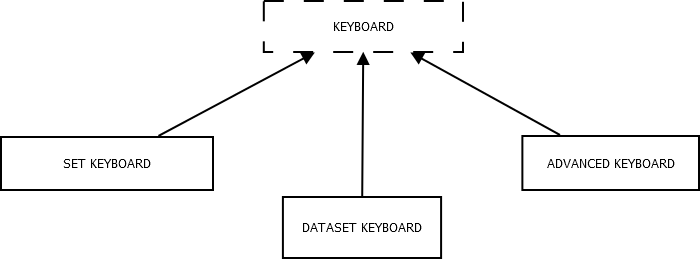
\includegraphics[scale=0.5]{img/Diagramma2.png}
			\caption{Gerarchia logica}
		\end{center}
	\end{figure}
    \subsubsection{Classe Keyboard}
    La gerarchia dei tastierini è determinata attraverso la classe astratta \textit{KeyBoard}, che deriva dalla classe \textit{QWidget}.
    Questa classe contiene i seguenti metodi virtuali puri:
    \begin{itemize}
        \item \textbf{std::vector<QString> getSingleOperationkeyboard()const}: ritorna un vettore contenente i nomi delle operazioni che utilizzano un solo operando;
        \item \textbf{std::vector<QString> getMultiOperationkeyboard()const}: ritorna un vettore contenente i nomi delle operazioni che utilizzano due operandi;
        \item \textbf{std::vector<QString> getExtraOperationkeyboard()const}: ritorna un vettore contenente i nomi delle operazioni che utilizzano un solo operando.
    \end{itemize}
    Queste rappresentano le tre principali famiglie di operazioni disponibili nella calcolatrice.
    Dispone inoltre di un metodo proprio:
        \begin{itemize}
            \item \textbf{void configure()}: configura il tastierino chiamando dinamicamente i metodi sopra citati e crea ed inserisce i tasti, questi poi vengono predisposti, attraverso delle \textit{connect} e dei \textit{SignalMapper}, per invocare dei segnali qualora cliccati.
        \end{itemize}
    Dispone dei seguenti segnali:
        \begin{itemize}
            \item \textbf{void multioperation(int)}: segnale che invia l'indice dell'operazione tra due \textit{Numbers};
            \item \textbf{void singleOperation(int)}: segnale che invia l'indice dell'operazione da seguire su di un\textit{Numbers};
            \item \textbf{void extraoperation(int)}: segnale che invia l'indice dell'operazione da eseguire;
        \end{itemize}

    \subsubsection{Classe SetKeyboard,DatasetKeboard,AdvancedKeboard}
    Le classi \textit{SetKeyboard},\textit{DatasetKeyboard} e \textit{AdvancedKeyboard} sono utilizzate per definire quali operazioni per il tipo di dato rispettivamente \textit{Set},\textit{Dataset} e \textit{Advanced} sia possibile eseguire.
    Vengono definite tre tipi di operazioni principali, i cui nomi vengono definiti all'interno di questi metodi:
    \begin{itemize}
        \item \textbf{std::vector<QString> getSingleOperationkeyboard()const}: ritorna un vettore contenente i nomi delle operazioni che utilizzano un solo operando;
        \item \textbf{std::vector<QString> getMultiOperationkeyboard()const}: ritorna un vettore contenente i nomi delle operazioni che utilizzano due operandi;
        \item \textbf{std::vector<QString> getExtraOperationkeyboard()const}: ritorna un vettore contenente i nomi delle operazioni che non ricadono nelle precedenti due famiglie;
        
    \end{itemize}

    \subsection{Gerarchia della logica}
    \begin{figure}[!h]
		\begin{center} 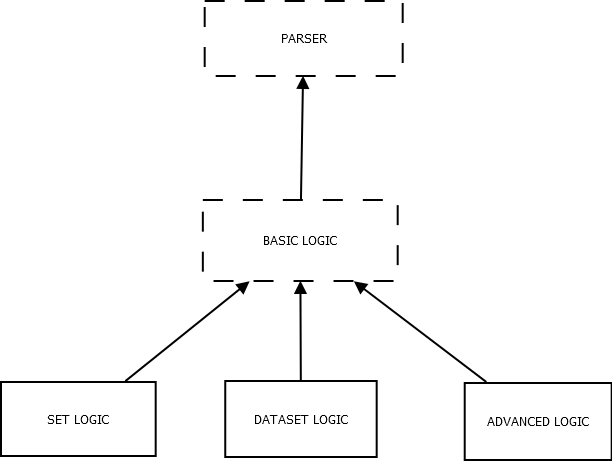
\includegraphics[scale=0.5]{img/Diagramma1.png}
			\caption{Gerarchia logica}
		\end{center}
	\end{figure}
    La gerarchia della logica è formata da una classe base atratta \textit{Parser}, da cui deriva una classe base atratta \textit{BasicLogic} da cui derivano tutte le classi concrete della logica come \textit{SetLogic}, \textit{DatasetLogic} e \textit{AdvancedLogic}.
        
        \subsubsection{Classe Parser}
        La classe base astratta \textit{Parser} permette di eseguire un \textit{parsing} delle stringhe prese in input, definisce un metodo virtuale puro con il seguente contratto:
        \begin{itemize}
            \item \textbf{bool condition()const}: ritorna \textit{true} se le condizioni di \textit{parsing} sono state rispettate altrimenti ritorna \textit{false}.
            \item \textbf{QString getNameType()}: ritorna il tipo dinamico dell'oggetto d'invocazione come una stringa;
        \end{itemize}
        Inoltre definisce i seguenti metodi:
        \begin{itemize}
            \item \textbf{std::list<int> parserData(QString)}: prende in input una \textit{QString} e se il \textit{parsing} va a buon fine restituisce una \textit{std::list<int>} contenente gli interi individuati dal parser;
            \item \textbf{std::string parserName(QString)}: prende in input una \textit{QString} e se è corrisponde al carattere "" gli riassegna il nome nome del tipo di dato dinamico e un intero positivo progressivo;
            \item \textbf{void restoreDefault()}: reimposta a valori di default i campi dati privati della classe.
        \end{itemize}
        
        \subsubsection{Classe BasicLogic}
        La classe \textit{BasicLogic} permette di eseguire le principali operazioni di base della calcolatrice, ha un campo dati di tipo \textit{std::list<Numbers*>*} al cui interno sono presenti oggetti di tipo statico \textit{Numbers} e tipo dinamico uno qualsiasi della gerarchia.
        Definisce inoltre diversi metodi virtuali puri con i seguenti contratti:
        \begin{itemize}
            \item \textbf{numbers* getObjectLogicClass(std::string,std::list<int>)}: ritorna un oggetto di tipo statico \textit{Numbers} costruito con suddetti parametri.
        \end{itemize}

        Inoltre definisce i seguenti metodi virtuali:
        \begin{itemize}
            \item \textbf{void clearKalkElements()}: elimina tutte le occorrenze nella lista generale di oggetti \textit{Numbers} con \textit{name() == getNameType()}.
            \item \textbf{void SetOperand(std::string, std::string )}: inserisce il nome dell'operando rispettivamente o nel primo o nel secondo operando;
            \item \textbf{void multioperation(int)}: fissa quale operazione multi insieme ci si aspetta e si attende il secondo operando;
            \item \textbf{void selectOperand(QListWidgetItem*)}: selezionea il nome dell'operando e si richiama il metodo \textit{SetOperand(std::string,std::string)};
            \item \textbf{void singleOperation(int)}: fissa quale operazione multi insieme ci si aspetta ed esegue l'operazione;
            \item \textbf{void add\_set(QString,QString)}: crea e successivamente aggiunge nella lista generale di oggetti \textit{Numbers} l'oggetto restituito dal metodo \textit{getObjectLogicClass(...,...)} dopo aver parsato le QStirng in input;
            \item \textbf{void sub\_set(QString)}: sottrae dalla lista generale di oggetti \textit{Numbers} quello con nome corrispondete al parametro QString e con tipo dinamico corrispondente a \textit{getNameType()}, altrimenti lancia un'eccezione;
            \item \textbf{void add\_elements(QString,QString)}: aggiunge gli interi dati dalla lista \textit{parserData(...)} all'oggetto \textit{Numbers} con nome corrispondente al primo parametro e stesso \textit{getNameType()} altrimenti lancia un'eccezione;
            \item \textbf{void add\_set(QString,QString)}: sottrae gli interi dati dalla lista \textit{parserData(...)} all'oggetto \textit{Numbers} con nome corrispondente al primo parametro e stesso \textit{getNameType()} altrimenti lancia un'eccezione;
            \item \textbf{void results()}: se non è disponibile nessun risultato lancia un'eccezione altrimenti lo inserisce nella lista generale di \textit{Numbers}.
        \end{itemize}

        Sono disponibili i seguenti metodi:
        \begin{itemize}
            \item \textbf{QString getNameType()}: restituisce il campo dati \textit{nameType} che rappresenta il tipo di dato dinamico a cui è inizializzata la \textit{BasicLogic};
            \item \textbf{bool checkType(std::string)const}: restituisce \textit{true} se i tipi di dato dinamici sono uguali \textit{false} altrimenti;
            \item \textbf{void AC()}: resetta gli operandi, l'operazione e il risultato corrente;
            \item \textbf{void getElements()}: emette un segnale con cui invia una \textit{std::list<QString>} con i nomi dei tipi di dato per cui checkType(...) ritorna \textit{true};
            \item \textbf{void update()}: metodo richiamato quando avviene un cambio di tipo di dato, aggiorna la lista di oggetti disponibili, chiude eventuali finestre di input aperte;
        \end{itemize}
        Dispone anche di segnali con i quali notificare o inviare richieste di informazioni o di modifica.

        \subsubsection{Classe SetLogic}
        La classe \textit{SetLogic} permette di eseguire le operazioni riguardanti il tipo di dato \textit{Set}, dispone principalmente dei seguenti metodi:
        \begin{itemize}
            \item \textbf{void singleOperation(int)}: esegue l'operazione data dal parametro int;
            \item \textbf{void add\_set(QString,QString)}: crea un nuovo oggetto se non ne esiste già uno con nome uguale e aggiunge la sua lista di interi al \textit{Set} "U";
            \item \textbf{void sub\_set(QString)}: Elimina l'oggetto \textit{Set} dalla lista di oggetti e sottrae il contenuto da "U" se non è contenuto in nessun'altro \textit{Set}, verifica ciò grazie alla funzione \textit{bool in(const int,std::string)const};
            \item \textbf{void add\_elements(QString,QString)}: aggiugne la lista di interi al \textit{Set} con nome ricercato e al \textit{Set} "U";
            \item \textbf{void sub\_elements(QString,QString)}: sottrae la lista di interi al \textit{Set} con nome ricercato e al \textit{Set} "U";
            \item \textbf{set* getObjectLogicClass(std::string,std::list<int>)}: ritorna un \textit{Set} costruito con i parametri;
            \item \textbf{void results()}: esegue l'operazione data dal parametro dagli operandi e dall'operazione precedentemente fissati;
            \item \textbf{void extraoperation(int)}: esegue l'operazione data dal parametro int;
        \end{itemize}

        \subsubsection{Classe DatasetLogic}
        La classe \textit{DatasetLogic} permette di eseguire le operazioni riguardanti il tipo di dato \textit{Dataset}, dispone dei seguenti metodi:
        \begin{itemize}
            \item \textbf{void singleOperation(int)}: esegue l'operazione data dal parametro int;
            \item \textbf{bool condition()const;}: condizione con cui si personalizza il parsing;
            \item \textbf{dataset* getObjectLogicClass(std::string,std::list<int>)}: ritorna un \textit{Dataset} costruito con i parametri;
        \end{itemize}

        \subsubsection{Classe AdvancedLogic}
        La classe \textit{AdvancedLogic} permette di eseguire le operazioni riguardanti il tipo di dato \textit{Advanced}, dispone dei seguenti metodi:
        \begin{itemize}
            \item \textbf{void singleOperation(int)}: esegue l'operazione data dal parametro int;
            \item \textbf{bool condition()const;}: condizione con cui si personalizza il parsing;
            \item \textbf{advanced* getObjectLogicClass(std::string,std::list<int>)}: ritorna un \textit{Advanced} costruito con i parametri;
        \end{itemize}

        \section{Classi contenitore AppKalk}
        La classe \textit{AppKalk} è la classe contenitore generale che permette contiene al suo interno 3 oggetti di tipo:
        \begin{itemize}
            \item \textbf{Logic}: gestore della logica;
            \item \textbf{Input}: gestore dell'input;
            \item \textbf{View}: gestore della vista;
        \end{itemize}
        \subsection{Classe Logic}
        La classe \textit{Logic} permette lo scambio del tipo di dato tra \textit{Set},\textit{Dataset} e \textit{Advanced} a livello logico e gestisce tutte le operazioni dei diversi tipi di dato, deriva dal tipo di dato \textit{QObject}.
        Possiede un campo dati di tipo \textit{std::vector<BasicLogic*>} detta \textit{Logics} per lo store delle unità logiche.
        Definisce poi un \textit{std::list<const numbers*>*} detto \textit{Uset} che viene passato per riferimento alle singole unità logiche che opereranno con condivisione di memoria, sarà poi compito della classe \textit{Logic} distruggere suddetta lista.
        Definisce un campo \textit{BasicLogic*} detto \textit{uni} rappresentante un riferimento all'unità logica corrente.
        Definisce i seguenti metodi SLOT:
        \begin{itemize}
            \item \textbf{void AC()}: invoca su \textit{uni} il metodo \textit{void AC()};
            \item \textbf{void multioperation(int)}: invoca su \textit{uni} il metodo \textit{void multioperation(int)};
            \item \textbf{void singleOperation(int)}: invoca su \textit{uni} il metodo \textit{void AC()};
            \item \textbf{void selectOperand(QListWidgetItem*)}: invoca su \textit{uni} il metodo \textit{void singleOperation(int)};
            \item \textbf{void changeLogic(int)}: assegna a \textit{uni} la logica nella posizione data dal parametro dentro \textit{logics};
            \item \textbf{void executeOperation(int,QString,QString)}: esegue un'operazione di input invocando su \textit{uni} i metodi \textit{add\_set(QString,Qstring)}, \textit{sub\_set(QString)}, \textit{add\_elements(QString,Qstring)}, \textit{sub\_elements(QString,Qstring)};
            \item \textbf{void clearKalkElements()}: invoca su \textit{uni} il metodo \textit{void changeLogic(int)};
            \item \textbf{void extraoperation(int)}: invoca su \textit{uni} il metodo \textit{void extraoperation(int)};
        \end{itemize}
        Definisce anche i seguenti metodi:
        \begin{itemize}
            \item \textbf{void setLogics()}: popola \textit{logics} inserendo le unità logiche;
            \item \textbf{std::vector<QString> nameType()const}: restituisce un vettore contenente \textit{QString} con tutti i nomi dei tipi di dato;
        \end{itemize}
        \subsection{Classe View}
        La classe \textit{View} permette lo scambio del tipo di dato tra \textit{Set},\textit{Dataset} e \textit{Advanced} a livello di vista, deriva dal tipo di dato \textit{QWidget}.
        Possiede una serie di campi da dati che fanno a formare la GUI, di seguito la lista:
        \begin{itemize}
            \item \textbf{int currentStatus}: indice della vista corrente;
            \item \textbf{QPalette* pal}: QPalette per colorare il QPushButton corrispondente al tipo di dato che si sta utilizzando;
            \item \textbf{QTextEdit* Barra}: sulla Barra verranno stampati tutti i messaggi che non siano errori, è situata nella parte alta;
            \item \textbf{QLineEdit* errori}: sulla barra degli errori verranno stampati tutti gli errori dovuti a tutte le operazioni tranne quelli dovuti ad errate operazioni di input;
            \item \textbf{QListWidget* elenco}: elenco su cui verrano mostrati gli oggetti \textit{Set},\textit{Dataset} e \textit{Advanced} disponibili;
            \item \textbf{QHBoxLayout* kalk}: kalk è il contenitore di tutti i widget;
            \item \textbf{std::vector<QPushButton*> statusButton}: :contenitore dei pulsanti della barra dei pulsanti di status;
            \item \textbf{std::vector<Keyboard*> views}: vettore con le i tastierini dei diversi tipi di dato.
        \end{itemize}
        Definisce i seguenti metodi SLOT:
        \begin{itemize}
            \item \textbf{void refresh(std::list<QString>)}: aggiorna l'Elenco degli oggetti disponibili;
            \item \textbf{void setAC()}: All Clear invia un segnale con cui resetta gli operandi, le operazioni e ripulisce la Barra;
            \item \textbf{void setBarra(QString)}: setta la Barra con il parametro \textit{QString};
            \item \textbf{void setError(QString)}: setta la barra degli errori con il parametro \textit{QString};
            \item \textbf{void changeLogic(int)}: emette un segnale con cui cambia l'unità logica e cambia anche il tastierino;
            \item \textbf{void changePallet(int)}: resetta il pulsante con la QPalette standard e setta con Pal il pulsante corrispondente al nuovo tipo corrente;
            \item \textbf{void clear()}: ripulsice Barra e barra degli errori;
        \end{itemize}
        Definisce anche i seguenti metodi:
        \begin{itemize}
            \item \textbf{void setViews()}: popola \textit{logics} inserendo i tastierini;
            \item \textbf{std::vector<QString> getBasicOperation()const}: restituisce un vettore contenente \textit{QString} le etichette per i pulsanti di operazione di input;
        \end{itemize}

        \subsection{Classe Input}
        La classe \textit{Input} permette lo di eseguire l'input delle informazioni con cui costruire gli oggetti utilizzati poi dalla calcolatrice.
        Possiede una serie di campi da dati che fanno a formare il pannello di input, di seguito la lista:
        \begin{itemize}
            \item \textbf{int operation}: indice dell'operazione di input;
            \item \textbf{bool isUsed}: \textit{true} allora esiste già un pannello di input, altrimenti \textit{false};
            \item \textbf{extrapanel* input\_view}: puntatore ad un pannello di input;
            \item \textbf{QMessageBox* MessageError}: pannello con messaggio d'errore per input che generino un errore;
        \end{itemize}
        Definisce i seguenti metodi SLOT:
        \begin{itemize}
            \item \textbf{void manageInput(int)}: imposta il pannello secondo l'operazione richiesta;
            \item \textbf{void unlock()}: sblocca il pannello di input;
            \item \textbf{void SendDataInput(QString,QString)}: invia gli input ricevuti;
            \item \textbf{void setErrorInput(QString)}: crea una QMessageBox ad esplicitare l'errore incorso;
            \item \textbf{void ifExistClose()}: se esiste chiude il pannello di input corrente;
        \end{itemize}
        Definisce anche i seguenti metodi:
        \begin{itemize}
            \item \textbf{void configureExtrapanel()}: permette di configurare il tastierino secondo l'operazione richiesta;   .       
        \end{itemize}

        \section{Descrizione del codice polimorfo}
        Nelle diverse classi precedentemente descritte sono presenti non pochi metodi che eseguono chiamate polimorfe.
        Per fare esempi di chiamate polimorfe ogni chiamata fatta dalla classe \textit{AppKalk} sul campo dati \textit{uni} è polimorfa, il tipo statico del puntatore è di tipo \textit{BasicLogic} mentre l'oggetto puntato potrebbe essere di tipo \textit{SetLogic},\textit{DatasetLogic} o \textit{AdvancedLogic}.
        Altri esempi di chiamate polimorfe possono essere individuati nella classe \textit{BasicLogic} nelle operazioni di input, dopo vengono chiamati i metodi \textit{add\_list} ed altri.

        \section{Estensibilità}
        \subsection{Prerequisiti}
        Questa sezione si propone di essere una guida all'estensione della calcolatrice con ulteriori tipi di dato, per prima cosa diciamo che il nuovo tipo di dato deve estendere la classe \textit{Numbers}, implementando i suoi metodi virtuali puri.
        Il nuovo tipo di dato può anche estendere una delle classi già disponibili eseguendo l'override dei metodi disponibili.
        Il nuovo tipo di dato potrà essere una sequenza di numeri interi.
        \subsection{Simmetria View\-Logic}
        Quando si inserisce il tastierino e l'unità logica nei rispettivi vettori assicurarsi che si trovino allo stesso indice assoluto.
        \subsection{View}
        La view del nuovo tipo di dato consisterà nel creare una classe derivata dalla classe \texit{Keyboard} implementando i tre metodi virtuali puri:
        \begin{itemize}
            \item std::vector<QString> getSingleOperationkeyboard()const: inserire qui i nomi delle operazioni singole;
            \item std::vector<QString> getSingleOperationkeyboard()const: inserire qui i nomi delle operazioni multiple;
            \item std::vector<QString> getSingleOperationkeyboard()const: inserire qui i nomi delle operazioni extra.
        \end{itemize}
        Per ciascuno di questi metodi si inizializzerà un vettore contenente QString, si procederà a \textit{pushare} al suo interno i nomi delle operazioni, l'ordine con cui verranno inserite sarà l'ordine in cui verranno chiamate nella parte logica. Da questo momento tutti i pulsanti sono già connessi nella parte logica, \\
        Ora spostiamoci nella classe \textit{View}, nel metodo \textit{void setViews()}, pushate in coda il nuovo tastierino appena creato.
        \subsection{Logica}
        Per indrodurre il nuovo tipo di dato nella calcolatrice dovrà essere creata una classe derivata dalla classe \textit{BasicLogic}, che dovrà estendere almeno i metodi virtuali puri:
        \begin{itemize}
            \item \textbf{numbers* getObjectLogicClass(QString,QString)}: ritornare un dato costruito con i parametri del tipo di dato che si gestisce; 
            \item \textbf{QString getNameType()}: il nome del tipo di dato che si gestisce;
            \item \textbf{bool condition()const}: condizioni personalizzazione del parsing;
        \end{itemize}
        Se si volesse inserire delle operazioni multiple, singole o extra, si dovrà procede all'override dei seguenti metodi:
        \begin{itemize}
            \item \textbf{void singleOperation(int index)}: operazione per i tipi di dato singoli;
            \item \textbf{void results()}: operazione per i tipi di dato multipli;
            \item \textbf{void extraOperation(int index)}: operazione per i tipi di dato singoli, vanno inserite le operazioni in ordine 
        \end{itemize}
        Le operazioni vanno inserite nello stesso ordine con cui sono stati inseriti i pulsanti nel tastierino.

        \section{Manuale utente}
        \subsection{Avvio}
        All’avvio dell’applicazione Kalk questa si troverà nella scheda \textit{Set}, per gli altri tipi di dato basterà premere i tasti in alto a destra cambiando così tipo di dato.
        \subsection{Struttura}
        La calcolatrice è divisa in tre aree principali: nell’area sulla sinistra è presente una lista che in base al tipo di dato su cui si sta lavorando mostra tutti gli insiemi creati fino a quel momento, la seconda parte è a sua volta divisa in altre quattro parti: nella parte superiore è presente un campo di output su cui vengono visualizzati gli insiemi selezionati e i risultati delle operazioni, nella parte immediatamente inferiore sono presenti due pulsanti, uno etichettato \textit{ClearKalk} per il reset della calcolatrice per quel tipo di dato, uno etichettato \textit{AC} per desettare gli operandi e l'operazione selezionata, nella parte centrale è presente un tastierino con quattro tasti con le operazioni di input, immediatamente sotto sono presenti una serie di pulsanti sui quali viene riportata una etichetta con l’operazione corrispondente.\\
        Infine nella parte inferiore è presente una barra di output dove verranno mostrati eventuali errori dovuti a operazioni non disponibili o a irregolarità nella costruzione di un insieme numerico.
        \subsection{Tipo dato corrente}
        Il tipo di dato corrente della calcolatrice è indicato in alto a destra dal pulsante di colore più scuro.
        Nella terza ed ultima parte, a destra della calcolatrice, sono presenti tre pulsanti con i quali è possibile cambiare lo status, premendo uno dei pulsanti la scheda verrà aggiornata al tipo selezionato. 
        \subsection{Dinamica operazioni}
        La dinamica di selezione di operandi e operazioni è la stessa che in una normale calcolatrice: 
        \begin{itemize}
            \item per effettuare operazioni tra due insiemi, si seleziona il primo insieme e successivamente l’operazione. Da questo momento non sarà più possibile cambiare il primo operando se non premendo il pulsante AC, che resetterà l’operazione corrente. Scelta l’operazione si procede scegliendo il secondo operando e premendo il pulsante "=", verrà quindi stampato a schermo il risultato indicando anche l’operazione corrispondente. Nel caso di errori o irregolarità verrà riportato l’errore corrispondente nella barra inferiore;
            \item Per operazioni di calcolo su singolo insieme, basta selezionare l’insieme su cui si vuole fare l’operazione e subito dopo l’operazione corrispondente; restituirà il risultato nella barra superiore;
            \item Per operazioni di manipolazione di insiemi: creazione o eliminazione di insiemi, modifica dei valori di un insieme, selezionare il pulsante corrispondente e seguire la procedura indicata nella finestra che comparirà.

        \end{itemize}

        **La scheda Set rende disponibile fin da subito un set chiamato “U”, questo è l’insieme universo dove sarà possibile vedere tutti gli elementi inseriti in ogni Set della scheda. Non è possibile eseguire operazioni su questo insieme se non quelle di inserimento o rimozione di valori, se si inserisce un valore questo resterà “spaiato”, se si elimina un valore dall’universo verrà rimosso da tutti i Set in
        cui compariva.
        Set rende disponibile anche una operazione di salvataggio del risultato corrente, la quale salva il risultato
        nella barra sulla sinistra e la rende disponibile per ulteriori operazioni.

        \section{Ore utilizzate}
        Sono state utilizzate le seguenti ore alla consegna:
        \begin{itemize}
            \item \textbf{Progettazione}: 2 ore;
            \item \textbf{Scrittura codice gerarchia tipi}: 0.30 ore;
            \item \textbf{Scrittura codice logica di controllo}: 10 ore;
            \item \textbf{Scrittura codice parte grafica}: 10 ore;
            \item \textbf{Scrittura relazione}: 4 ore;
            \item \textbf{Test}: 2 ore;
            \item \textbf{Traduzione gerarchia tipi in Java}: 0.30 ore.

        \end{itemize}
        \section{Ambiente di sviluppo}
        \begin{itemize}
            \item Sistema operativo: Ubuntu 16.04.3 LTS
            \item Compilatore: gcc version 5.4.0 20160609
            \item QT: 5.9.3
            \item QMake version 2.01a
        \end{itemize}
\end{document}